% Szkielet dla pracy inżynierskiej pisanej w języku angielskim.

\documentclass[english,bachelor,a4paper,twoside]{ppfcmthesis}

\usepackage[utf8]{inputenc}
\usepackage[OT4]{fontenc}
\usepackage[T1]{fontenc}
\usepackage{graphicx}
\usepackage{listings}
\usepackage{xcolor}
\usepackage{pifont}

\newcommand*\OK{\ding{51}}

\definecolor{codestrings}{rgb}{0.164,0,1}
\definecolor{codecomment}{rgb}{0.25,0.49,0.37}
\definecolor{codekeywords}{rgb}{0.8,0,0.33}
\definecolor{codebackground}{rgb}{0.95,0.95,0.95}
\lstdefinestyle{cblockstyle}{
	inputencoding=utf8,
	language=C++,
	extendedchars=true,
	basicstyle=\ttfamily\footnotesize,
	numbers=left,
  	numbersep=3pt,
	framexleftmargin=2pt,
  	framerule=0pt,
  	frame=lines,
	numberstyle=\tiny,
	tabsize=2,
	showstringspaces=false,
	showspaces=false,
	  keywordstyle=\bfseries\color{codekeywords},
	  identifierstyle=\color{black},
	  stringstyle=\color{codestrings},
	  commentstyle=\color{codecomment},
	  columns=fullflexible,
	  abovecaptionskip=\medskipamount,
	  belowcaptionskip=\medskipamount,
	  backgroundcolor=\color{codebackground},
}
\lstdefinestyle{pblockstyle}{
	inputencoding=utf8,
	language=python,
	extendedchars=true,
	basicstyle=\ttfamily\footnotesize ,
	numbers=left,
  	numbersep=3pt,
	framexleftmargin=2pt,
  	framerule=0pt,
  	frame=lines,
	numberstyle=\tiny,
	tabsize=2,
	showstringspaces=false,
	showspaces=false,
	  keywordstyle=\bfseries\color{codekeywords},
	  identifierstyle=\color{black},
	  stringstyle=\color{codestrings},
	  commentstyle=\color{codecomment},
	  columns=fullflexible,
	  abovecaptionskip=\medskipamount,
	  belowcaptionskip=\medskipamount,
	  backgroundcolor=\color{codebackground},
}
\lstdefinestyle{clinestyle}{
	tabsize=2,
	frame=lines,
	inputencoding=utf8,
	language=C++,
	keywordstyle=\bfseries\color{codekeywords},
	identifierstyle=\color{black},
	stringstyle=\color{codestrings},
	commentstyle=\color{codecomment},
	basicstyle=\ttfamily,
}
\lstnewenvironment{cblock}{\lstset{style=cblockstyle}}{}
\lstnewenvironment{clinee}{\lstset{style=clinestyle}}{}
\lstnewenvironment{pblock}{\lstset{style=pblockstyle}}{}
\graphicspath{ {figures/} }

% Authors here.
\author{%
   Michał Kempka \album{105256} \and 
   Grzegorz Runc \album{109759} \and 
   Jakub Toczek \album{109704} \and 
   Marek Wydmuch \album{109746}}
\authortitle{}                                        % Do not change.
\title{VIZIA: 3D Video Game-based Environment for Research on Learning Agents from Raw Visual Information}        % Note how we protect the final title phrase from breaking (~zamiast spacyj)
\ppsupervisor{~Wojciech Jaśkowski,~Ph.~D.} % Your supervisor comes here.
\ppyear{2016}                                         % Year of final submission (not graduation!)

\begin{document}
\lstset{breaklines=true,
    postbreak=\raisebox{0ex}[0ex][0ex]{\ensuremath{\color{red}\hookrightarrow\space}}}
% Front matter starts here
\frontmatter\pagestyle{empty}%
\maketitle\cleardoublepage%

% Blank info page for "karta dyplomowa"
\thispagestyle{empty}\vspace*{\fill}%
\begin{center}Tutaj przychodzi karta pracy dyplomowej;\\oryginał wstawiamy do wersji dla archiwum PP, w pozostałych kopiach wstawiamy ksero.\end{center}%
\vfill\cleardoublepage%

%Streszczenie i abstrakt
\chapter*{Streszczenie}

Niniejsza praca jest poświęcona wykorzystaniu trójwymiarowych gier typu FPS (ang. first-person shooter) do badań nad inteligentnymi agentami, które działają i uczą się w oparciu o informację obrazową.

W ciągu ostatnich lat komputery znacznie przewyższyły ludzi pod względem możliwości prze-twarzania surowych danych.
Nie dotyczy to jednak przetwarzania informacji obrazowej, w przypadku której postęp dotyczy tylko ograniczonych zastosowań.
Konwolucyjne sieci neuronowe z powodzeniem są wykorzystywane do klasyfikacji zdjęć, a w połączeniu z uczeniem ze wzmocnieniem znajdują zastosowanie m.in. w robotyce.
Głębokie uczenie ze wzmocnieniem zostało również wykorzystane do nauczenia agenta grania w 7 gier z Atari 2600.
Przestrzeń praktycznych zastosowań jest jednak w tym przypadku ograniczona, ponieważ jest to informacja obrazowa o dwuwymiarowym charakterze.
Dodanie aspektu głębi, a zatem wykorzystanie gier trójwymiarowych, znacznie zwiększyłoby możliwość praktycznych zastosowań.
Ze względu na obserwowanie świata z perspektywy pierwszej osoby szczególnie interesujące pod tym względem wydają się być gry FPS, jednak dotychczas nie prowadzono badań nad wykorzystaniem uczenia ze wzmocnieniem z informacji obrazowej pochodzącej z gry FPS.

Celem pracy było opracowanie łatwego w użyciu środowiska do badań nad inteligentnymi agentami, które działają i uczą się w oparciu o informację obrazową generowaną przez trójwymiarową grę FPS, oraz przeprowadzenie eksperymentów dla prostych scenariuszy.

Rezultatem niniejszej pracy jest środowisko VIZIA oparte na grze Doom dostosowane do potrzeb paradygmatu uczenia ze wzmocnieniem.
Stworzony został interfejs programistyczny zaimplementowany w C++ pozwalający na wykonywanie akcji, pobieranie obrazu i informacji o bohaterze gry, jak i swobodny dobór parametrów wykonania gry.
Parametry te mogą być zapisywane w postaci plików konfiguracyjnych.
Zapewniono również wsparcie dla Pythona i Javy.
Środowisko to wspiera tworzenie scenariuszy testowych w zewnętrznych edytorach i implementację funkcji nagrody za pomocą języka skryptowego Action Code Script.
Poza trybem pełnej kontroli nad grą zaimplementowano również tryb obserwatora, pozwalający na uczenie agenta na podstawie rozgrywki prowadzonej przez człowieka.
Dodatkowo środowisko może pracować w trybie zarówno synchronicznym, w którym gra czeka na akcje agenta, jak i asynchronicznym, w którym gra działa ze stałą prędkością, co pozwala na wykorzystanie jej w rozgrywkach sieciowych.

Stworzone oprogramowanie zostało przygotowane do pracy w systemie Linux i udostępnia tryb niewymagający środowiska graficznego, dzięki czemu może być uruchamiane na zdalnych stanowiskach.
Środowisko umożliwia przetwarzanie z prędkościami liczonymi w tysiącach klatek na sekundę.

Przeprowadzone dla prostych środowisk testowych eksperymenty wykorzystujące uczenie ze wzmocnieniem głębokich sieci neuronowych wskazują na użyteczność stworzonego środowiska do badań nad głębokim uczeniem ze wzmocnieniem z informacji obrazowej.
	

\chapter*{Abstract}

This thesis is concentrated on usage of 3-dimensional FPS games in research on intelligent agents that act and learn based on purely visual information.


In the last couple of years computers significantly exceeded humans in terms of raw data processing.
It does not apply, however, to visual information processing, which has been equally successful only for certain applications.
Convolutional Neural Networks are successfully used for image classification, and combined with reinforcement learning they prove to be useful in robotics, among others.
Deep reinforcement learning has also been employed to teach an intelligent agent to play 7 Atari 2600 games.
However, range of practical applications of such technology is very limited, as it works with visual input which is two-dimensional.
Adding the depth, thus involving games in three-dimensional environments, would notably increase real-life practicality.
Due to first-person perspective, First-person shooter games (FPS) are especially interesting. However, no research has been conducted so far, that involves reinforcement learning from raw visual data generated by an FPS game.

The main aim of this thesis was to create an easy-to-use environment for research on intelligent agents that act and learn based on purely visual data generated by a three-dimensional FPS game, and conducting simple experiments for the most basic scenarios.


Work on this thesis resulted in creation of environment employing a vintage game --- Doom to expose an interface proper for reinforcement learning --- VIZIA. VIZIA's application programming interface was fully written in C++ and allows making in-game actions, retrieve game's screen buffer and plenty of in-game parameters such as player's health or ammunition. 
The API offers a myriad of configuration options which can easily be written and stored in text files.
In addition to C++ support bindings for Python and Java has been created as these languages are more popular for AI research purposes. 
The environment offers a mechanism of scenarios that enables researchers to design custom research conditions that support reinforcement learning paradigm.
What is more, multiple different modes of operation are available and allow taking full control over game's engine processing, perform apprenticeship learning or even engage in multiplayer/multiagent skirmishes. 

VIZIA is mainly targeted at Linux platform and provides options for off-screen rendering that requires no graphical environment, therefore can be used with remote terminals.
The environment allows reaching processing speeds counted in thousands of frames per second.

In order to test practicality of using VIZIA in AI research, a simple experiment has been conducted that in fact proves that the environment serves its purpose.

\cleardoublepage

% Table of contents.
\pagenumbering{Roman}\pagestyle{ppfcmthesis}%
\tableofcontents* \cleardoublepage%

% Main content of your thesis starts here.
\mainmatter%



\chapter{Introduction}
\label{ch:introduction}
\section{Motivation}
\label{sec:motivation}

Visual signals are one of the main sources of information about the surrounding environment for humans and animals.
While computers have already greatly exceeded humans in terms of raw data processing, they still do not match their ability to process images.
However, recent increase in computing power and emergence of affordable technologies allowing to perform general computations on graphics cards (CUDA, OpenCL) enabled a significant progress in this area.
An important part of this advance are deep convolutional neural networks (CNNs).


CNNs for the first time came into prominence when they were used to classify 1.6 millions images into 1000 classes~\cite{NIPS2012_4824}.
This solution was so effective that now this is the prevalent method of image classification.
This success hugely popularized CNNs and soon enough they were used for much more complex tasks.
In combination with reinforcement learning, they were used to model intelligent agent which attempted playing 7 Atari 2600 games from Arcade Learning Platform\cite{mnih-atari-2013}.
In 6 of them the achieved results were better than in all of the previous approaches, and in the case of 3 results were better than those achievable by human players.

The main drawback of Atari games is that they are only two-dimensional, so their usability at solving real-world problems is quite limited, but reinforcement learning itself was successfully used for identifying features in static images \cite{conf/cvpr/GoodrichA12} and in robotics for controlling racing slot car using only image from the camera \cite{rieijcnn12} and even for steering RC helicopter\cite{Abbeel07anapplication}.
Bigger scope of practical applications is offered by 3D games which are a better approximation of the real-world.
% <---
Among 3D games, First Person Shooter (FPS) games are particularly interesting because the first-person perspective is a good equivalent of the image obtained from the mobile robot vision systems.
Also important is their great popularity, and simple game rules make it easy to implement rewarding mechanism.
% >---

FPS games have already been successfully used in research on artificial intelligence, especially the most popular ones such as Unreal Tournament \cite{6314567} \cite{6922494}, Counter-Strike \cite{5035619} or Quake III Arena \cite{el2007hybrid}.
However, in these studies agents acted upon high-level information like positions of walls, enemies, locations of item etc, which are normally inaccessible to human player.
Supplying only raw visual information would relieve researchers of the burden of supplying AI high-level information and handcrafted features.
What is more it would force agents to become more autonomous and behave in a way more resembling real intelligent agents (humans and animals).
So far no studies have been conducted on the reinforcement learning from visual information obtained from 3D FPS games.


Currently there are no environments that allow using FPS games for research on artificial intelligence algorithms, in which agents rely exclusively on raw visual information.
This could be a serious factor that is impending the progress of visual information-based research on reinforcement learning.
Engaging in that kind of research would require a large amount of work associated with creation of an environment integrating game engine with interface suited to reinforcement learning paradigm.
The existence of such a tool would allow to conduct experiments and focus on the goal of research without having to worry about availability of the test environments.
 

\section{Aims and scope}
%%W rozdziale 1 nie pojawia sie nazwa VIZIA
The main aim of this thesis is, thus Section~\ref{sec:motivation}, to create an easy to use and flexible environment for research on intelligent agents that work and learn using the raw visual information generated by the engine of 3D FPS game. 
% <---
In order to confirm usability of the created environment experiments on simple scenarios should be conducted.
% >---

The goal will be achieved by meeting the following objectives:
\begin{itemize}
 \item to compare and select needed technologies,
 \item to implement the environment,
 \item define API,
 \item to define and implement test scenarios in the created environment,
 \item to implement learning algorithms for deep neural networks,
 \item to conduct experiments for simple test scenarios.
\end{itemize}
% <---
It was assumed that VIZIA environment has to meet the following assumptions:


\begin{enumerate}
\item based on popular open-source 3D FPS game (ability to modify the code and the freedom of publication)
\item lightweight (portability and the ability to run multiple instances)
\item fast (AI should be a limiting factor for the speed of processing, not the game itself)
\item total control over game's processing (pausing processing for the duration of AI run)
\item customizable resolution and rendering parameters (adjusting the image generated by the game to meet the needs)
\item multiplayer (testing agent in the fight against the human player or other AI)
\item spectator mode (agent learning from observations of a human playing)
\item easy and convenient creation of custom scenarios (creating test environments tailored to the needs)
\item reinforcement learning friendly API in C++ (use for the research on reinforcement learning; the ability to bind other languages)
\item Python bindings (popularity of Python in machine learning)
\item multiplatform (availability of full functionality on Linux, Windows and Mac OS)
\end{enumerate}

% >---

%The created environment should be based on open-source, lightweight 3D FPS game that allows total control over game's processing and customising resolution and rendering parameters.
%There should be implemented spectator mode, in which agent can learn from observations of a human playing.
%Support for easy and convenient creation of custom scenarios should be essential part of the environment. 
%Designed API should be reinforcement learning friendly and implemented in C++ with bindings to Python and possibly other languages (Java, Lua etc.)
%The environment should be multiplatform, focused on Linux, with Windows and OS X support.

%Brakuje o multiplayer i o tym, ze ma byc szybkie (powod).
%To jest bardzo wazny paragraf i chcialbym, zeby go rozwinac. Niech bedzie sie zaczynal od tego, ze przyjeto, ze srodowisko ma spelniac nastepujace zalozenia. I tutaj punktowana lista zalozen: 1) based on open-source (powod), 2) lightweight (powod)...	
	
\section{Thesis organization}


This thesis is structured as follows. 
Chapter~\ref{ch:architecture} gives an overview of technologies and tools used to develop the VIZIA environment and describes environment's architecture. It addresses design decisions and problems and contains result of performance tests. 
Chapter~\ref{ch:api} presents the designed application programming interface, python binding and shows API's usage examples. 
Chapter~\ref{ch:scenarios} gives definition of scenario and presents tools and methods for creating scenarios. It contains the description of designed scenarios. 
Chapter~\ref{ch:experiment} shows methods used for conducting experiments and their results. 
Chapter~\ref{ch:conclusions} concludes this thesis and proposes directions for future work.

\section{Contributions}
	\subsection{Engineering Project}
	\begin{description}
		\item[Michał Kempka] \hfill
			\begin{itemize}
				\item part of interface design,
				\item testing and experiments,
				\item part of python binding,
				\item python examples,
				\item scenarios creation,
				\item support for configuration files.
			\end{itemize}
		\item[Grzegorz Runc] \hfill
			\begin{itemize}
				\item generation of depth buffer,
				\item support for off-screen rendering.
			\end{itemize}
		\item[Jakub Toczek] \hfill
			\begin{itemize}
				\item python binding,
				\item java binding.
			\end{itemize}
		\item[Marek Wydmuch] \hfill
			\begin{itemize}
				\item VIZIA API design,
				\item VIZIA API and VIZIADoomModule implementation,
				\item CMake configuration.
			\end{itemize}
	\end{description}
	
   	
	\subsection{Thesis}
	\begin{description}
		\item[Michał Kempka] \hfill
			\begin{itemize}
				\item foundations for Chapter \ref{ch:api},
				\item Chapter \ref{ch:scenarios},
				\item Chapter \ref{ch:experiment},
				\item Chapter \ref{ch:conclusions},
				\item translation of the abstract.
			\end{itemize}
		\item[Grzegorz Runc] \hfill
			\begin{itemize}
				\item Chapter~\ref{ch:introduction},
				\item Section~\ref{sec:technologies}.
                \item the abstract
			\end{itemize}
		\item[Jakub Toczek] \hfill
			\begin{itemize}
				\item Chapter~\ref{ch:api}.
			\end{itemize}
		\item[Marek Wydmuch] \hfill
			\begin{itemize}
				\item Section~\ref{sec:architecture},
				\item Section~\ref{sec:architecture_solutions},
				\item Section~\ref{sec:performance}.
			\end{itemize}
	\end{description}


\chapter{Framework Outline}

\section{Used Technologies}
What we used and why.
\begin{itemize}
\item zdoom, mention alternatives
\item linux focus, cpp core, python wrapper
\item acs scripting in doombuilder 2 for scenarios
\item python and lasagne for experiments
\end{itemize}

\section{Architecture}
Nice diagram (in DOOM style) with the arcitecture.
\begin{itemize}
\item Zdoom separate process.
\item Boost interprocess: shared memory to comunicate with zdoom.
\item Flow control and PLAYER vs SPECTATOR mode.
\item Warnings and exceptions.
\end{itemize}

\section{Problems and Solutions}
\begin{itemize}
\item Why shared memory and separate doom process and what it entails.
\item Why make/set action are like they are. Why action is a vector not just number.
\item Why state is copied in Python but not in cpp.
\item Zbuffer struggles.
\item Why Windows and Mac are not supported so well.
\item Why scenario is effectively divided into config file nad doom iwad file.
\item Why multiplayer is barely usable.
\end{itemize}

\section{Performance}
Table with some fps ratings and a graph.
Conclusions: it's fast enough, any reasonably good AI will be much slower during learning process.

\section{Building process}
\subsection{Prerequisites}
\begin{itemize}
\item preferably linux
\item cmake
\item make
\item gcc 4.??
\item boost v ?
\item python 2.6 with numpy (v?) for pyhon wrapper
\item java ? for java wrapper
\item ...
\end{itemize}
\subsection{Compilation}
cmake, make and they lived happily ever after



\chapter{Application Programming Interface}
\section{Methods}
	\subsection{Configuration}
	Methods described below are setting the main parameters of the environment, such as resolution of the generated image or Intelligent Agent's available actions. They should be invoked before the init() method. Any attempt to invoke them after initialization will result in a warning/exception depending on severity of consequences. 
	\vspace{20pt}

		\begin{clinee}
		DoomGame();
		\end{clinee}

Constructor that creates an instance of the game. Zdoom is not ready for action after the constructor, it needs further initialization. Object is inicialized with the following values:
	\begin{itemize}
\item Resolution: 640x480
\item Game path: ./viziazdoom
\item Game iwad path: "./doom2.wad"
\item Map: map01 (first map created in the iwad file if it's not changed purposefully)
\item Mode: PLAYER
\item GameVariables: none
\item CustomGameArg: none
\item Available buttons: ATTACK, USE, JUMP, CROUCH, SPEED, MOVE\_RIGHT, MOVE\_LEFT, MOVE\_BACKWARD, MOVE\_FORWARD, TURN\_RIGHT, TURN\_LEFT
\item Rendering: All
\item Window: displayed 
\item DoomSkill: ??????????
\item Co z tymi autostartami i rewardami?
	\end{itemize}


\vspace{20pt}
\begin{clinee}
~DoomGame();
\end{clinee}

The destructor that safely ends the work of environment and removes the object.


\vspace{20pt}
\begin{clinee}
bool init();
\end{clinee}

Function which initializes enviroment. Configuration cannot be changed after invokation of init(). Dooms instance is created in separate process. Returns true when game was started properly. 


\vspace{20pt}
\begin{clinee}
bool loadConfig(std::string filename);
\end{clinee}

Loads and sets configuration from a configuration file. It's syntax is better described in Section~\ref{sec:configuration_file}. The configuration file can substitute any combination of the following methods call. In case of multiple invokations, they will overwrite selected settings from previous calls. Return true when all configuration was read properly.


\vspace{20pt}
\begin{clinee}
void addAvailableButton(Button button);
\end{clinee}

Adds support for the specified actions (e.g. TURN\_LEFT, MOVE\_FORWARD ). If no buttons are specified (the method is not called) 11 default buttons are added. Their list may be found in constructor description.


\vspace{20pt}
\begin{clinee}
void addAvailableButton(Button button, int maxValue);
\end{clinee}

Adds support for the specified actions responsible for rotation and sets the amount of movement done. It only applies to "buttons" responsible for rotation. it effectively constraints rotation speed. %TODO CO TO ROBI?!


\vspace{20pt}
\begin{clinee}
void setButtonMaxValue(Button button, int maxValue);
\end{clinee}

Sets the button's max value. It only applies to "buttons" responsible fors rotation and moving(with specified speed), it effectively constraints rotation/moving speed.
0 means no constraint and it's the default behavior TODO %TODO CO TO ROBI?!


\vspace{20pt}
\begin{clinee}
void addAvailableGameVariable(GameVariable var);
\end{clinee}

Adds given GameVariable to the list of values returned in getState() (e.g. AMMO1, HEALTH, ATTACK\_READY).


\vspace{20pt}
\begin{clinee}
void clearAvailableButtons();
\end{clinee}

Disables support for any specified buttons. It will result in default setting which can be found in constructor description.


\vspace{20pt}
\begin{clinee}
void clearAvailableGameVariables();
\end{clinee}

Clears the list of game variables returned in getState().


\vspace{20pt}
\begin{clinee}
void addCustomGameArg(std::string arg);
\end{clinee}

Adds a custom argument for the zdoom process. %TODO OPIS


\vspace{20pt}
\begin{clinee}
void clearCustomGameArgs();
\end{clinee}

Clears all arguments specified by addCustomGameArg().


\vspace{20pt}
\begin{clinee}
void setMode(Mode mode);
\end{clinee}

Sets mode in which the game will be started. Supported formats are defined in Mode enumaration (e.g. PLAYER, SPECTATOR).


\vspace{20pt}
\begin{clinee}
void setDoomGamePath(std::string path);
\end{clinee}

Sets path to zdoom executable.


\vspace{20pt}
\begin{clinee}
void setDoomIwadPath(std::string path);
\end{clinee}

Sets path to the game iwad file.


\vspace{20pt}
\begin{clinee}
void setDoomFilePath(std::string path);
\end{clinee}

Sets path to additional iwad file (e.g. scenario).


\vspace{20pt}
\begin{clinee}
void setDoomMap(std::string map);
\end{clinee}

Sets map to be used by doom.


\vspace{20pt}
\begin{clinee}      
void setDoomSkill(int skill);
\end{clinee}

Sets doom game difficulty level (0-5) which is called skill in doom. Less means easier. It affects ammo, life amount and monster aggressiveness. %TODO co tutaj? 


\vspace{20pt}
\begin{clinee}
void setDoomConfigPath(std::string path);
\end{clinee}

Sets path for doom configuration file.


\vspace{20pt}
\begin{clinee}    
void setEpisodeStartTime(unsigned int tics);
\end{clinee}

Sets start delay of every episodes in doom tics. Every episode will effectively start (from the user's perspective) after given number of tics.


\vspace{20pt}
\begin{clinee}
void setEpisodeTimeout(unsigned int tics);
\end{clinee}

Sets quantity of tics after which the episode will be finished.


\vspace{20pt}
\begin{clinee}
void setLivingReward(double livingReward);
\end{clinee}

Sets the reward granted for player being alive after each tic.


\vspace{20pt}
\begin{clinee}
void setDeathPenalty(double deathPenalty);
\end{clinee}

Sets penalty for player's death. In case of negative value, player will be rawarded for each decease.


\vspace{20pt}
\begin{clinee}
void setAutoNewEpisode(bool set);
\end{clinee}

Determines if automatic episode restart will be set in case of the end of previous one.


\vspace{20pt}
\begin{clinee}
void setNewEpisodeOnTimeout(bool set);
\end{clinee}

Determines if automatic episode restart will be set in case of the timeout.


\vspace{20pt}
\begin{clinee}
void setNewEpisodeOnPlayerDeath(bool set);
\end{clinee}

Determines if automatic episode restart will be set in case of players death.


\vspace{20pt}
\begin{clinee}
void setNewEpisodeOnMapEnd(bool set);
\end{clinee}

Determines if automatic episode restart is set when player reaches the end of the map.


\vspace{20pt}
\begin{clinee}
void setScreenResolution(ScreenResolution resolution);
\end{clinee}

Sets screen resolution. Supported resolutions are part of ScreenResolution Enumeration type and their format is: RES\_xXy (e.g. RES\_320X240, RES\_1920X1080). Buffer as well as content of zdoom's window is affected.


\vspace{20pt}
\begin{clinee}
 void setScreenFormat(ScreenFormat format);
\end{clinee}

Sets format of the screen buffer. Supported formats are defined in ScreenFormat enumaration (e.g. CRCGCB, RGB24, GRAY8). Content displayed in zdoom's window what change no matter which format you choose - it only affects the buffer.


\vspace{20pt}
\begin{clinee}       
void setRenderHud(bool hud);
void setRenderWeapon(bool weapon);
void setRenderCrosshair(bool crosshair);
void setRenderDecals(bool decals);
void setRenderParticles(bool particles);
\end{clinee}

Methods that determine if some elements (hud, weapon, crosshair, decals, particles) will be displayed.


\vspace{20pt}
\begin{clinee}
void setWindowVisible(bool visibility);
\end{clinee}

Determines if zdoom's window will be visible.
Turning it off will result in:
\begin{itemize}
\item Linux - rendering and any computations connected with the window will be skipped. It results in processing acceleration
\item Windows - window will be hided. No processing acceleration
\end{itemize}


\vspace{20pt}
\begin{clinee}
void setConsoleEnabled(bool console);
\end{clinee}

Determines if zdoom's and vizia's console output will be displayed (e.g. "You picked up a medpack", "Player killed himself.", "Vizia\_init ....")


\vspace{20pt}
\subsection{Runtime}
The following methods handles gameplay. They directly affect the game and should be used after inicialization. 
Any attempt to invoke them before it will result in a warning/exception depending on severity of consequences. 


\vspace{20pt}
\begin{clinee}
void newEpisode();
\end{clinee}

Initializes new episode. All rewards, map state etc are restarted.


\vspace{20pt}
\begin{clinee}
	void setAction(std::vector<int> &actions);
\end{clinee}

Sets the player's behavior in the next tic.
Each vector's value corresponds to button specified with addAvailableButton() function (in invocation order).
In case of possitive value, picked action will be triggered with the specified strength. Descrete actions (e.g. ATTACK) will be performed once.


\vspace{20pt}
\begin{clinee}
	void advanceAction();
\end{clinee}

Method performs a tic using action obtained by setAction(). After function call, action vector is not reseted and will be performed once again if not changed.


\vspace{20pt}
\begin{clinee}
	void advanceAction(bool stateUpdate, bool renderOnly, unsigned int tics);
\end{clinee}

Method performs a given number of tic in the row. Descrete actions (e.g. ATTACK) will be only performed in the first tic, analog actions (moving, turning) will be repeated every tic. 
Function also determines if state should be updated. What's more, setting renderOnly option as true will disable buffer update. Hovewer, it will not affect zdoom main window.  


\vspace{20pt}
\begin{clinee}
	double getLastReward();
\end{clinee}

Returns the reward from last advanceAction. If a single action lasted longer then one tick, function it will return cumulative reward from all tics.


\vspace{20pt}
\begin{clinee}
	double makeAction(std::vector<int> &actions);
\end{clinee}

Function combining usibility of setAction(), advanceAction() and getLastReward(). It sets the player's behavior in the next tic, performe one and returns reward.
Each vector's value corresponds to button specified with addAvailableButton() function (in invocation order).
In case of possitive value, picked action will be triggered with the specified strength. Descrete actions (e.g. ATTACK) will be performed once. 


\vspace{20pt}
\begin{clinee}
	double makeAction(std::vector<int> &actions, unsigned int tics);
\end{clinee}

Function combining usibility of setAction(), advanceAction() and getLastReward(). It sets the player's behavior in the next number of tics given to the function, performes it and returns cumulative reward from all tics. Each vector's value corresponds to button specified with addAvailableButton() function (in invocation order). Descrete actions (e.g. ATTACK) will be only performed in the first tic, analog actions (moving, turning) will be repeated every tic with given strength.
State will be updated after that. Buffer will not be updated.


\vspace{20pt}
\begin{clinee}
	State getState();
\end{clinee}

Returns struct State with the current game state. More detailed description of the struct can be found in Section~\ref{sec:structs}.


\vspace{20pt}
\begin{clinee}
	std::vector<int> getLastAction();
\end{clinee}

Returns a vector with the last action performed. Each vector's value corresponds to button specified with addAvailableButton() function (in invocation order). Most usefull in SPECTATOR mode.


\vspace{20pt}
\begin{clinee}
	uint8_t * const getGameScreen();
\end{clinee}

Returns the screen buffer. Values depend on the settings set befor inicialization. The same value may be found in State structure. Its length is returned in getScreenPitch() function.


\vspace{20pt}
\begin{clinee}
	int getGameVariable(GameVariable var);
\end{clinee}

Returns value of the specified game variable (AMMO1, HEALTH etc.). It does not need to be a value returned in State.
It could be used for e.g. shaping. Returns 0 in case of not finding given GameVariable.


\vspace{20pt}
\begin{clinee}
	double getSummaryReward();
\end{clinee}

Returns sum of all rewards gathered in the current episode.


\vspace{20pt}
\begin{clinee}
	bool isNewEpisode();
\end{clinee}

Checks if the current episode is in the initial state. Returns true if no tic was performed.


\vspace{20pt}
\begin{clinee}
	bool isEpisodeFinished();
\end{clinee}

Checks if the current episode is in the terminal state. Returns true if the episode has ended. No makeAction/advanceAction functions should be called after this point.


\vspace{20pt}
\begin{clinee}
	void setSeed(unsigned int seed);
\end{clinee}

Sets the seed of the randomizing engine. Using the same seed and actions in another episode will affect in reproducing the gameplay.


\vspace{20pt}
\begin{clinee}
	void close();
\end{clinee}

Closes zdoom engine and corresponding processes. Metod frees used resources (memory allocations e.t.c). It is automatically invoked by destructor - should be used only when closing zdoom engine in the middle of processing is needed.


\vspace{20pt}
\begin{clinee}
	bool isRunning();
\end{clinee}

Checks if the current zdoom process is running.


\vspace{20pt}
\begin{clinee}
	void sendGameCommand(std::string cmd);
\end{clinee}

Sends a given command to zdoom console. Can be used for cheats, multiplayer e.t.c.


\vspace{20pt}
\subsection{QUERY INTERFACE}


Api provides a number of getters associated with the above-mentioned functions and a set of additional methods to help converts units.
  

\vspace{20pt}
\begin{clinee}
int getAvailableButtonsSize();
int getAvailableGameVariablesSize();
Mode getMode();
double getLivingReward();
double getDeathPenalty();
unsigned int getEpisodeStartTime();
unsigned int getEpisodeTimeout();
unsigned int getEpisodeTime();
int getScreenWidth();
int getScreenHeight();
int getScreenChannels();
size_t getScreenPitch();
size_t getScreenSize();
ScreenFormat getScreenFormat();
unsigned int getSeed();
int getButtonMaxValue(Button button);
\end{clinee}


\paragraph {Metods} Metods outsite the DoomClass:


\begin{clinee}
unsigned int DoomTics2Ms(unsigned int tics);
\end{clinee}

Function calculating number of milliseconds during given tics.


\vspace{20pt}
\begin{clinee}
unsigned int Ms2DoomTics(unsigned int ms);
\end{clinee}

Function calculating how many tics will be made during given number of milliseconds.


\vspace{20pt}
\begin{clinee}
double DoomFixedToDouble(int doomFixed);
\end{clinee}

DO OPISANIA


\vspace{20pt}
\section{Structures and Enumerations} \label{sec:structs}
\subsection{State}


Structure created to store all the information needed by inteligent agent to process the image.  
It is composed of three public fields:

\vspace{20pt}	
\begin{clinee}
	struct State {
	    unsigned int number; 
	    std::vector<int> gameVariables;
	    uint8_t * imageBuffer;
	};
\end{clinee}
number - Number of the state in the current episode. (tic number?)\\
gameVariables - vector storing user-defined, during the configuration, values drawn from the game such as AMMO or HEALTH 
imageBuffer - pointer to the screen buffer, containing the image information.
\begin{itemize}
\item struct state
\item enumeration types . . .or maybe move it to the apendinx?
\end{itemize}
\subsection{Mode}
Enumeration used to set the general game mode.
Posible values:
\begin{itemize}
\item PLAYER - 
\item SPECTATOR -
\item ASYNC\_PLAYER -
\item ASYNC\_SPECTATOR -
\end{itemize}
\subsection{ScreenFormat}
Enumeration used to set the general game mode.
\begin{itemize}
 \item CRCGCB 
 \item CRCGCBZB
 \item RGB24
 \item RGBA32
 \item ARGB32
 \item CBCGCR
 \item CBCGCRZB
 \item BGR24
 \item BGRA32
 \item ABGR32
 \item GRAY8
 \item ZBUFFER8
 \item DOOM\_256\_COLORS
\end{itemize}
\subsection{ScreenResolution}
\begin{itemize}
\item RES\_40X30,
 \item      RES\_60X45,
 \item       RES\_80X50,
 \item       RES\_80X60,
 \item       RES\_100X75,
 \item       RES\_120X75,
 \item       RES\_120X90
 \item       RES\_160X100,
 \item      RES\_160X120,
      \item  RES\_200X120,
      \item  RES\_200X150,
      \item  RES\_240X135,
      \item  RES\_240X150,
      \item  RES\_240X180,
      \item  RES\_256X144,
      \item  RES\_256X160,
      \item  RES\_256X192,
      \item  RES\_320X200,
      \item  RES\_320X240,
      \item  RES\_400X225,	// 16:9
      \item  RES\_400X300,
  \item      RES\_480X270,	// 16:9
 \item       RES\_480X360,
 \item       RES\_512X288,	// 16:9
 \item       RES\_512X384,
 \item       RES\_640X360,	// 16:9
 \item       RES\_640X400,
 \item       RES\_640X480,
 \item       RES\_720X480,	// 16:10
 \item       RES\_720X540,
 \item       RES\_800X450,	// 16:9
 \item       RES\_800X480,
 \item       RES\_800X500,	// 16:10
  \item      RES\_800X600,
 \item       RES\_848X480,	// 16:9
 \item       RES\_960X600,	// 16:10
 \item       RES\_960X720,
 \item       RES\_1024X576,	// 16:9
 \item       RES\_1024X600,	// 17:10
 \item       RES\_1024X640,	// 16:10
 \item       RES\_1088X612,	// 16:9
 \item       RES\_1152X648,	// 16:9
 \item       RES\_1152X720,	// 16:10
 \item       RES\_1152X864,
 \item       RES\_1280X720,	// 16:9
 \item       RES\_1280X854,
 \item       RES\_1280X800,	// 16:10
 \item       RES\_1280X960,
 \item       RES\_1280X1024,	// 5:4
 \item       RES\_1360X768,	// 16:9
 \item       RES\_1366X768,
 \item       RES\_1400X787,	// 16:9
 \item       RES\_1400X875,	// 16:10
 \item       RES\_1400X1050,
 \item       RES\_1440X900,
 \item       RES\_1440X960,
 \item       RES\_1440X1080,
  \item      RES\_1600X900,	// 16:9
 \item       RES\_1600X1000,	// 16:10
 \item       RES\_1600X1200,
 \item       RES\_1680X1050,	// 16:10
 \item       RES\_1920X1080,
 \item       RES\_1920X1200,
 \item       RES\_2048X1536,
 \item       RES\_2560X1440,
 \item       RES\_2560X1600,
 \item       RES\_2560X2048,
 \item       RES\_2880X1800,
 \item       RES\_3200X1800,
  \item      RES\_3840X2160,
 \item       RES\_3840X2400,
 \item       RES\_4096X2160,
  \item      RES\_5120X2880,
\end{itemize}
\subsection{GameVariable}
\begin{itemize}
\item KILLCOUNT,
\item        ITEMCOUNT,
\item        SECRETCOUNT,
\item        FRAGCOUNT,
\item        HEALTH,
\item        ARMOR,
\item        DEAD,
\item        ON\_GROUND,
\item        ATTACK\_READY,
\item        ALTATTACK\_READY,
 \item       SELECTED\_WEAPON,
\item      SELECTED\_WEAPON\_AMMO,
 \item       AMMO0,
\item        AMMO1,
\item        AMMO2,
\item        AMMO3,
 \item       AMMO4,
 \item       AMMO5,
 \item       AMMO6,
 \item       AMMO7,
\item       AMMO8,
\item        AMMO9,
 \item       WEAPON0,
 \item       WEAPON1,
\item        WEAPON2,
 \item       WEAPON3,
 \item       WEAPON4,
 \item       WEAPON5,
\item        WEAPON6,
\item        WEAPON7,
\item        WEAPON8,
\item        WEAPON9,
 \item       USER1,
 \item       USER2,
 \item       USER3,
 \item       USER4,
 \item       USER5,
\item        USER6,
\item        USER7,
\item        USER8,
\item        USER9,
\item        USER10,
\item        USER11,
\item        USER12,
\item        USER13,
\item        USER14,
\item        USER15,
\item        USER16,
\item        USER17,
\item        USER18,
\item        USER19,
\item        USER20,
\item        USER21,
\item        USER22,
\item        USER23,
\item        USER24,
\item        USER25,
\item        USER26,
\item        USER27,
\item        USER28,
\item        USER29,
\item        USER30,
\end{itemize}
\subsection{Button}
\begin{itemize}
\item ATTACK = 0,
\item         USE = 1,
\item         JUMP = 2,
\item         CROUCH = 3,
\item         TURN180 = 4,
\item         ALTATTACK = 5,
\item         RELOAD = 6,
\item         ZOOM = 7,

\item         SPEED = 8,
\item         STRAFE = 9,

\item         MOVE\_RIGHT = 10,
\item         MOVE\_LEFT = 11,
\item         MOVE\_BACKWARD = 12,
\item         MOVE\_FORWARD = 13,
\item         TURN\_RIGHT = 14,
\item         TURN\_LEFT = 15,
\item         LOOK\_UP = 16,
\item         LOOK\_DOWN = 17,
\item         MOVE\_UP = 18,
\item         MOVE\_DOWN = 19,
\item         LAND = 20,
        //SHOWSCORES 20

\item         SELECT\_WEAPON1 = 21,
\item         SELECT\_WEAPON2 = 22,
\item         SELECT\_WEAPON3 = 23,
\item         SELECT\_WEAPON4 = 24,
\item         SELECT\_WEAPON5 = 25,
\item         SELECT\_WEAPON6 = 26,
\item         SELECT\_WEAPON7 = 27,
\item         SELECT\_WEAPON8 = 28,
\item         SELECT\_WEAPON9 = 29,
 \item        SELECT\_WEAPON0 = 30,

\item     SELECT\_NEXT\_WEAPON = 31,
 \item        SELECT\_PREV\_WEAPON = 32,
\item         DROP\_SELECTED\_WEAPON = 33,

 \item        ACTIVATE\_SELECTED\_ITEM = 34,
 \item        SELECT\_NEXT\_ITEM = 35,
 \item        SELECT\_PREV\_ITEM = 36,
 \item        DROP\_SELECTED\_ITEM = 37,

 \item        LOOK\_UP\_DOWN\_DELTA = 38,
 \item        TURN\_LEFT\_RIGHT\_DELTA = 39,
 \item        MOVE\_FORWARD\_BACKWARD\_DELTA = 40,
 \item        MOVE\_LEFT\_RIGHT\_DELTA = 41,
 \item        MOVE\_UP\_DOWN\_DELTA = 42,
\end{itemize}
\section{Configuration file}\label{sec:configuration_file}


Configuration file stores group of parameters and initial settings for the future use. It can be loaded into the game before inicialization. Settings can be overwritten after that action, giving the possibility of changing sigle parameter without interference in the file itself. There should be met certain requirements as to its content and name to make it load successfully.

Name of the configuration file should be with .properties suffix.

Content of the file should be composed of keywords identifying the setting and the value assigned to it separated with '='. Keyword is constructed similarly to the setting name, for example: episodeStartTime, windowVisible. However, two of them differ: availablebuttons, availablegamevariables.
Keyword can be written in both underscore and camel notation (case-insensitive). 


Value should be placed after '=' sign. File paths should not be placed between "" marks like the rest of the string values.
\begin{cblock}
...
#Values
living_reward = -1
render_crosshair = false
#Path
doom_iwad_path = ../../scenarios/doom2.wad
doom_file_path = ../../scenarios/basic.wad
#Normal String
doom_map = "map01"
...
\end{cblock}
Enum values should be passed using their name.
\begin{cblock}
...
#Enums
screen_format = CRCGCB
mode = PLAYER
...
\end{cblock}
Each setting should be separated from each other by a sign of the new line. In order to improve readability, it's possible to add a comment line by adding a '\#' sign at the beginning of the new line.

An exceptionally behave here availablebuttons and availablegamevariables functions because instead of individual variables, take as an argument the list of values in '\{\}'. The individual components should be separated from each other by a newline.
\begin{cblock}
...
# Available buttons
available_buttons = 
	{ 
		MOVE_LEFT 
		MOVE_RIGHT 
		ATTACK 
	}
# Game variables that will be in the state
available_game_variables = { AMMO2}
...
\end{cblock}

\section{Wrappers}
\subsection{Python}

Python functions and metods are very similar to the c++ ones. Howewer, because of the language differences, some of the values may vary. All differences are listed below.

\paragraph {Naming}
Naming convention used in python binding is underscore. The only exception is the constructor which is named in the same way like in c++.

\begin{cblock}
c++: DoomFixedToDouble(int doomFixed)
python: doom_fixed_to_double(int doomFixed)
\end{cblock}


\paragraph {Structures}
 State is changed structuraly: bufer is a numpy array and game variables are contained in a Python list. Whats more, getState() copies the buffer and gameVariables what doesn't happen in cpp. 
\paragraph {Enumerations}
Python equivalent of enums were created with the same names.
\paragraph {Types}
Due to the languages differences, some types have been modified.
\begin{itemize} 
\item Vectors in all functions were changed to python lists of compatible type.

\item  uint8\_t, unsigned int, size\_t were changed to int
\end{itemize}



\subsection{Java}
Java, like python, is a bit different then c++. All differences and the most important principles of using are listed below.

\paragraph {Naming}
 Naming convention is camelcase 
\begin{clinee}
c++: DoomFixedToDouble(int doomFixed)
java: DoomFixedToDouble(int doomFixed)
\end{clinee}
\paragraph {Structures}
State is changed structuraly: bufer and game variables are int tables (int[]). Whats more, getState copies the buffer and gameVariables, it doesn't happen in cpp. 
\paragraph {Enumerations}
 Enumerations were created the same like in c++ (you have to use them like in java:)
\begin{clinee}
 dg.addAvailableButton(Button.ATTACK);
\end{clinee}
\paragraph {Types}
Due to the languages differences, some types have been modified.
\begin{itemize}
\item Vectors in all functions were changed to java tables of compatible type (vector<int> = int[]).
\item uint8\_t, unsigned int, size\_t were changed to int
\end{itemize}
\section{Extended Examples}


\chapter{Scenarios}

To allow researchers to evaluate learning agents in conditions of different characteristics, we provide a mechanism of scenarios.

In this chapter we define what a scenario is (see Section \ref{sec:scenario_definition}), describe sample scenarios included with the API (see Section \ref{sec:scenarios}) and point out essentials of creating custom scenarios (see Section \ref{sec:creating_scenarios}).

\section{Definition}\label{sec:scenario_definition}
	Scenarios are DOOM resource files in special iwad format. A single scenario defines a map (structure of the world e.g. walls, corridors, monsters) and~a~script which determines behavior of entities and events. The script is also the place to assign rewards for various events. A scenario can define multiple maps in one iwad and~they all can be accessed by the framework. Default name for a map is `map01' but in general it can be completely arbitrary. Each map requires a separate script file.
	\\
	Scenarios cannot affect:
	\begin{itemize}
		\item constraints regarding buttons that can and cannot be used,
		\item episode timeout,
		\item skill level (they can affect; however, everything that depands on it),
		\item any rendering options e.g. screen resolution or~crosshair visibility,
		\item engine's reaction to player's death.
	\end{itemize}

	Due to scenarios' ability to set rewards they could be used to implement so called \emph{living~reward} and a~penalty for dying. Nonetheless, using API's \emph{setLivingReward} and \emph{setDeathPenalty} methods (see //REFERENCE HERE//).

\section{Tools}\label{sec:tools}
	\begin{figure}
			\centering
			\includegraphics[scale=0.3]{slade.png}
			\caption{Slade 3 application for scenario creation.}\label{fig:slade}
		\end{figure}

	Creating iwad files involves compilation thus~requires a dedicated software. \emph{Slade~3} and \emph{Doom~Builder~2}  were our editors of choice because of huge popularity, availability of resources and~relative quality. The editors differ mostly in user interface details but~both provide most curcial functionalities:

	\begin{itemize}
		\item \textbf{visual map editor} - a simple tool for map creation which is very easy to use and~enables you to achieve whatever is possible in Doom engine.
		\item \textbf{Action Code Script support} - dedicated language resembling C that is suitable for determining behavior of any monster, player and~object in the game.
		\item \textbf{testrunning} - possibility to test your scenario without resorting to external software or~calls. Test running requires providing a \emph{zdoom} executive file and \emph{doom2.wad} file (or~any other basic resource file) . 
	\end{itemize}

	Both tools are robust, reasonably easy to use and~provide much elasticity in sceanrio creation. However, due to the lack of native \emph{Linux} support and~some bad design solutions (mainly concerning interface) we consider \emph{Doom~Builder~2} a slightly inferior choice. 

	\newpage
\section{Provided Scenarios}\label{sec:scenarios}
	Each subsection includes `Suggested configuration' which suggests additional configuration which can be achieved by loading	configuration from file or additional API methods (see Section /REF/). These particular are quite arbitrary and adjusting them to personal preferences is encouraged.

	\subsection{Basic}\label{subsec:basic}
		
		\begin{figure}
			\centering
			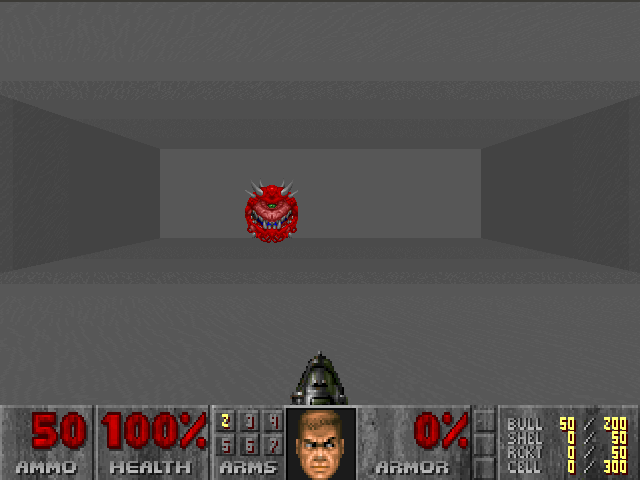
\includegraphics[scale=0.5]{basic.png}
			\caption{Doom gameplay frame from `basic' scenario.}\label{fig:basic}
		\end{figure}

		\paragraph{Motivation}
			Main purpose of this scenario is to show that Reinforcement Learning using only visual input is feasible using Vizia. The scenario is very simple but involves most fundamental mechanics of the game like shooting, movement and delays between actions and reactions of the world.
		
		\paragraph{Decription}
			The map is a rectangle with gray walls, ceiling and floor. Agent is spawned along the longer wall, in the center. A red, circular monster is spawned randomly somewhere along the~opposite wall. Agent can only (config) move left, move right and~shoot. 1 hit is enough to kill the~monster. Episode ends when the monster is killed or on timeout.
		
		\paragraph{Rewards}
			\begin{itemize}
				\item +101 for killing the monster
				\item -5 for missing
			\end{itemize}
		
		\paragraph{Suggested configuration}
			\begin{itemize}
				\item living reward = -1
				\item available buttons: move left, move right, shoot (attack)
				\item timeout = 300
			\end{itemize}
	\newpage

	\subsection{Deadly Corridor}
		\begin{figure}
			\centering
			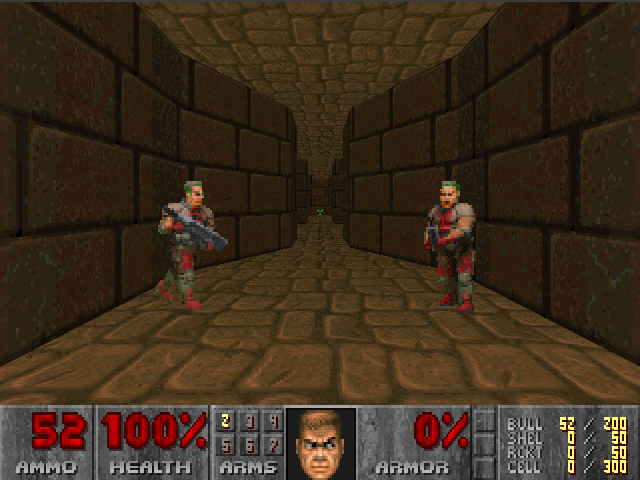
\includegraphics[scale=0.5]{deadly_corridor.png}
			\caption{Doom gameplay frame from `deadly corridor' scenario.}\label{fig:deadly_corridor}
		\end{figure}

		\paragraph{Motivation} 
			The purpose of this scenario is essentially to teach an agent be a responsible adult with good spacial orientation: focus efforts towards good direction and be able to sacrifice instant gratification in favour of future benefits and lifespan. Coping with the task requires some degree of spacial orientation and ability to see connection between monsters' presence and deteriorating health which, unattended, results in agent's death.

		\paragraph{Decription}
			The map is a corridor with shooting monsters on both sides (6 monsters in total). A green vest is placed at the oposite end of the corridor. Reward is proportional (negative or positive) to change of the distance between the player and the vest. If player ignores monsters on the sides and runs straight for the vest he will be killed somewhere along the way. To ensure this behavior \textit{doom\_skill} equal to 5 (config) is needed.

		\paragraph{Rewards}
			\begin{itemize}
				\item $\Delta$x for getting closer to(further from) the vest by $\Delta$x units in the corridor's axis of symmetry.
			\end{itemize}
			
		\paragraph{Suggested configuration}
			\begin{itemize}
				\item available buttons: turn left, turn right, move left, move right, shoot (attack)
				\item timeout = 4200
				\item death penalty = 100
				\item doom skill = 5
				\item availale game variables: HEALTH
			\end{itemize}
	\newpage

	\subsection{Defend the Center}\label{subsec:defend_the_center}
		\begin{figure}
			\centering
			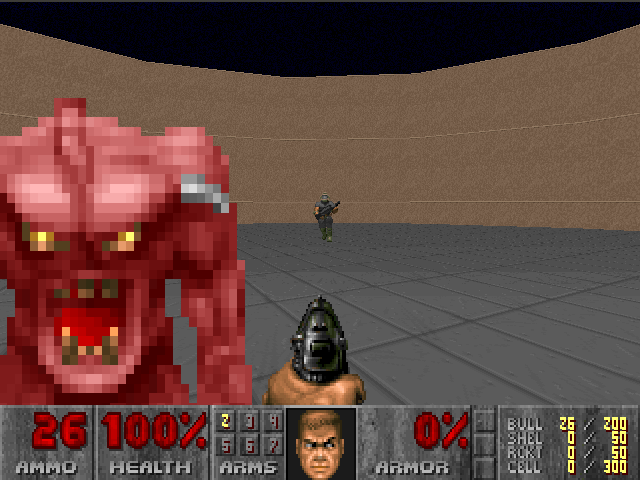
\includegraphics[scale=0.5]{defend_the_center.png}
			\caption{Doom gameplay frame from `defend the center' scenario.}\label{fig:basic}
		\end{figure}
		\paragraph{Motivation} 
			The purpose of this scenario is to encourage agents to develop some intuition about depth and awareness of potential danger coming from behind. Obviously, agents should also learn that monsters are sinister and killing them is rewarding, but it is not sufficient. Coincidentaly an agent could be expected to learn to impersonate a calissical Greek tragic hero: he is doomed to die pitifully (ammunition is finite) no matter his acions.

		\paragraph{Decription}
			The map is a large circle. Player is spawned in the exact center. 5 melee-only, monsters are spawned along the wall. Monsters are killed after a single shot. After dying each monster is respawned after some time. Episode ends when the player dies (it's inevitable becuse of limitted ammunition supplies).

		\paragraph{Rewards}
			\begin{itemize}
				\item +1 for killing a monster
			\end{itemize}
		
		\paragraph{Suggested configuration}
			\begin{itemize}
				\item death penalty = 1
				\item available buttons: turn left, turn right, shoot (attack)
				\item available game variables: HEALTH, AMMO2(pistol ammo)
			\end{itemize}
	\newpage

	\subsection{Defend the Line}
		\begin{figure}
			\centering
			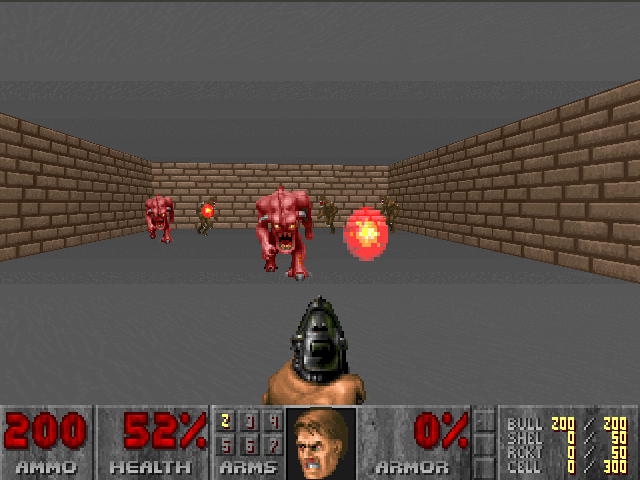
\includegraphics[scale=0.5]{defend_the_line.png}
			\caption{Doom gameplay frame from `defend the line' scenario.}\label{fig:defend_the_line}
		\end{figure}
		\paragraph{Motivation} 
			The purpose of this scenarios is to tech agents risk assessment and basic monster biology by presenting them with monsters of two types: melee and shoting. Agents should be able to recognize that shooters pose more imidiate threat than melee monster (unless they are at point blank range). Obviously, agents should also learn that monsters are sinister and killing them is rewarding, but it is not sufficient. Coincidentaly an agent could be expected to learn to impersonate a calissical Greek tragic hero: he is doomed to die pitifully (ammunition finite) no matter his acions.

		\paragraph{Decription}
			The map is a rectangle. Player is spawned along the longer wall, in the center. 3 melee and 3 shooting monsters are spawned along the oposite wall. Monsters are killed after a single shot, at first. After dying each monster is respawned after some time and can endure more damage. Episode ends when the player dies (it's inevitable becuse of limitted ammo).
		\paragraph{Rewards}
			\begin{itemize}
				\item +1 for killing a monster
			\end{itemize}

		\paragraph{Suggested configuration}
			\begin{itemize}
				\item available buttons: move left, move right, shoot (attack)
				\item death penalty = 1
				\item available game variables: HEALTH, AMMO2(pistol ammo)
			\end{itemize}
	\newpage

	\subsection{Deathmatch}
		\begin{figure}
			\centering
			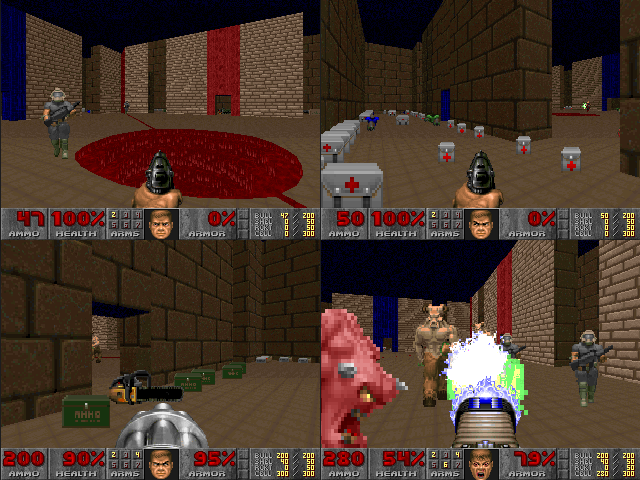
\includegraphics[scale=0.5]{deathmatch.png}
			\caption{4 Doom gameplay frames from `deathmatch' scenario.}\label{fig:deatchmatch}
		\end{figure}
		\paragraph{Motivation} 
	 		This scenario is a fully fledged fight for survival that should in effect create a virtual animal. Agent should be able to present effective understanding of many higher level concepts as fleeing, hiding, camping, resupplying, navigation or changing weapons to survive and kill a signifficant quantity of monsters.

		\paragraph{Decription}
			The map consists of a square room (hall) of considerable size and 4 small rooms (supply rooms) adjacent to each wall of the hall. 2 supply rooms contain signifficant quantity of medkits and armours. Other 2 contain a shotgun, chainsaw, plasma gun, chaingun, rocket launcher and ammunition. Agent is spawned in random location inside the hall. After a very short period monsters start to spawn in random locations of the hall. Monsters include shooters and melee brawlers. Agent is rewarded for killing monsters. Toughest mosters are less probable to appear and produce greater rewards.
		\paragraph{Rewards}
			\begin{itemize}
				\item +1/2/3/4/5/10 for killing a monster (exact value depands on monster type).
			\end{itemize}
		
		\paragraph{Suggested configuration}
			\begin{itemize}
				\item available buttons: all buttons coresponding movement, turning, shooting and weapon change 
				\item timeout = preffered finite value
				\item available game variables: HEALTH, ARMOR and all variables connected with weapons and ammo
			\end{itemize}		
	\newpage

	\subsection{Health Gathering}
		\begin{figure}
			\centering
			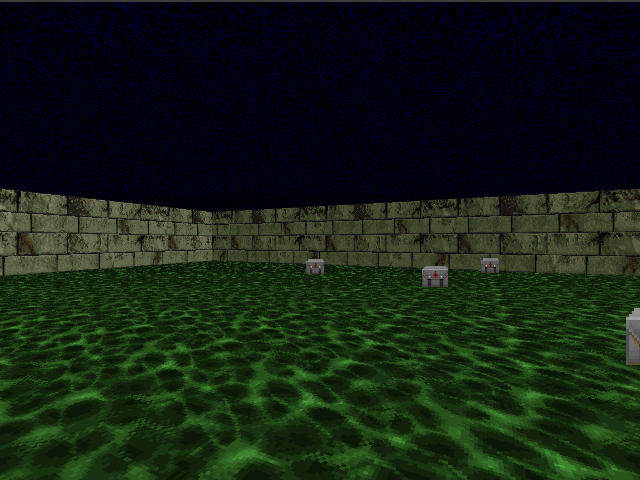
\includegraphics[scale=0.5]{health_gathering.png}
			\caption{Doom gameplay frame from `health gathering' scenario.}\label{fig:health_gathering}
		\end{figure}
		\paragraph{Motivation}
			The purpose of this scenario is to teach an agent that every second of his life is precious and collecting things increase his lifespan in this brutal world. The agent should be able to see that deteriorating health causes death and how walking into influences his health. It is advisable to equip the agent with some kind of memory because medkits that are directly in front of agent's feet cannot be noticed. In case of developing consciousness agent could deduce that there is a devine being in the skies that loves him and sends medkits to save him.

		\paragraph{Decription}
			The map is a rectangle with green, acidic floor which hurts players periodically. Deadliness of acid depands on skill level. Initially there are some medkits uniformly distributed over the map. New medkits fall from the skies peridically. A medkit heals some portions of player's health - to survive agent needs to pick them up. Episode finishes after player's death or on timeout.

		\paragraph{Suggested configuration}
		\begin{itemize}
			\item living reward = 1
			\item death penalty = 100
			\item available buttons: move left, move right, move forward
			\item timeout = 2100
			\item available game variable: HEALTH
		\end{itemize}
	\newpage

	\subsection{My Way Home}
		\begin{figure}
			\centering
			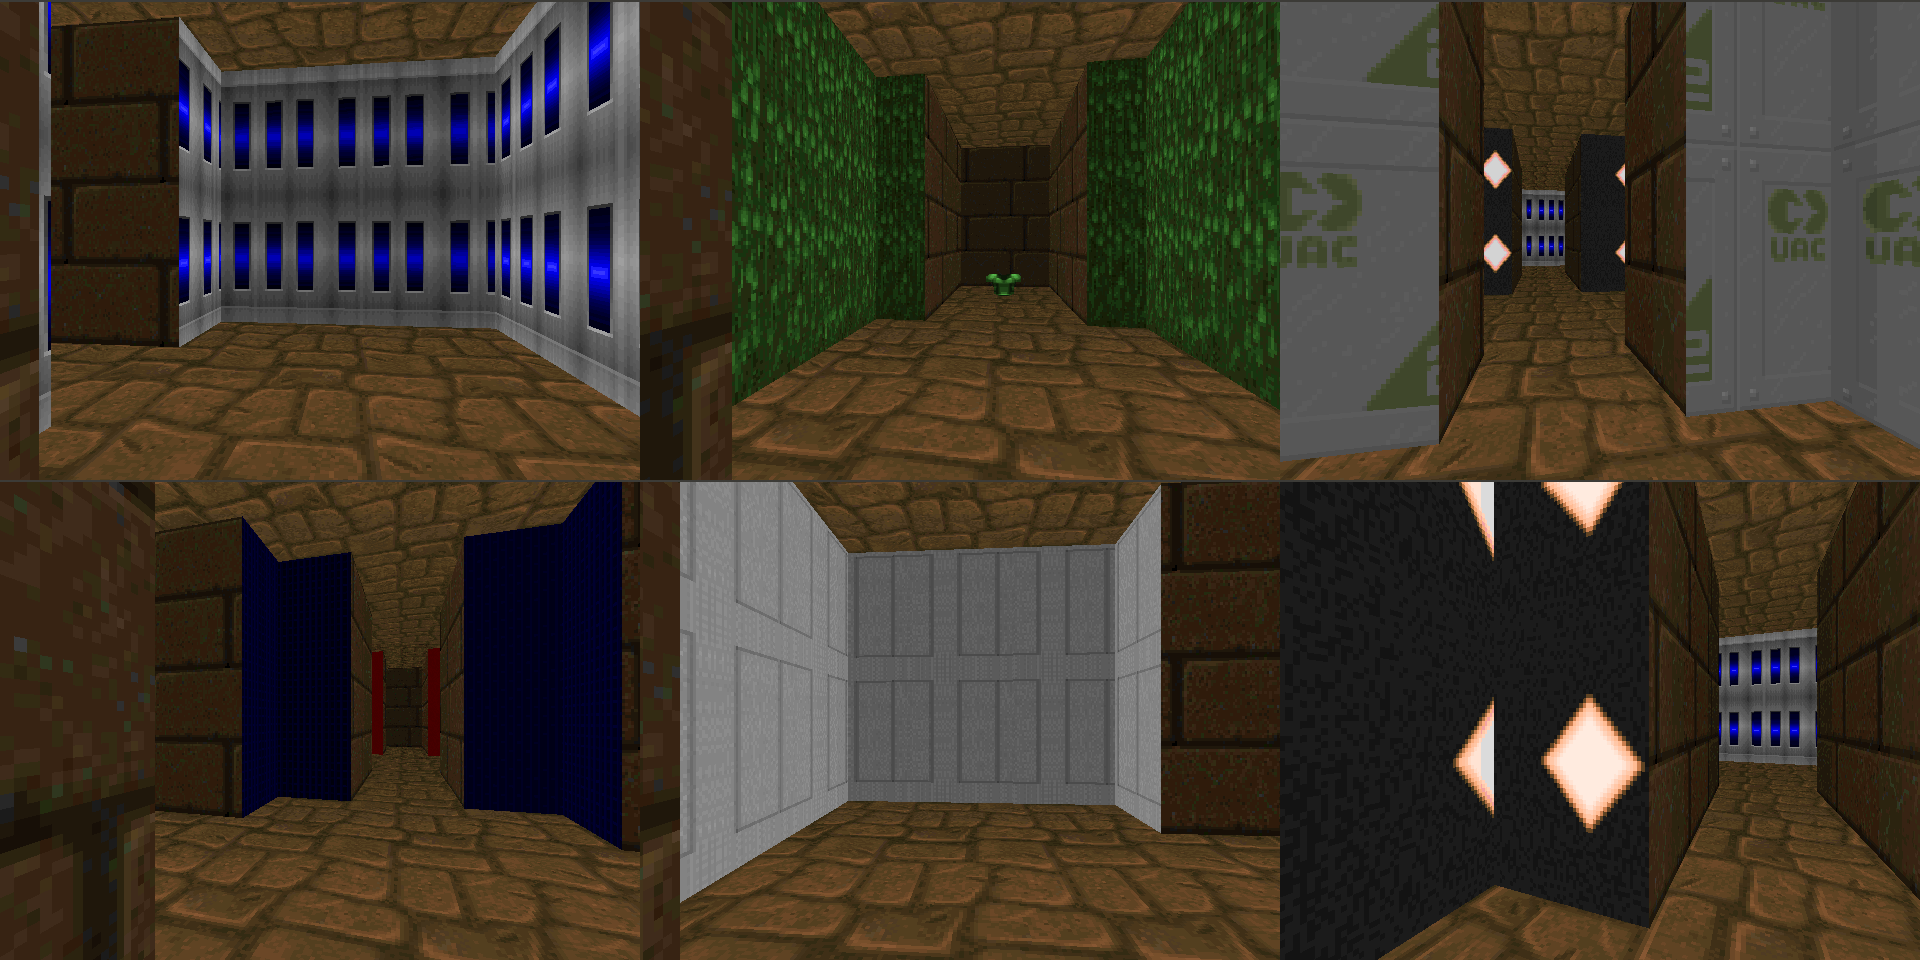
\includegraphics[scale=0.22]{my_way_home.png}
			\caption{6 Doom gameplay frames from `my way home' scenario.}\label{fig:my_way_home}
		\end{figure}
		\paragraph{Motivation} 
			The purpose of this scenario is to teach the agent how to navigate in a labirynth-like surroundings and reach his ultimate goal (and learn what the goal actually is). Agent should learn to determine his position in the maze and navigate.

		\paragraph{Decription}
			The map is a series of small rooms interconnected by short passages and 1 corridor with a dead end. Each room has a different color. A green vest is placed in one of the rooms (the same room every time). Player is spawned in randomly choosen room facing a random direction. Episode ends when the vest is reached or on timeout.
		\paragraph{Rewards}

		\begin{itemize}
			\item +1 for reaching the vest
		\end{itemize}
		
		\paragraph{Suggested configuration}
		\begin{itemize}
			\item living reward = -0.0001
			\item available buttons: move left, move right, shoot (attack)
			\item timeout = 2100
		\end{itemize}
	\newpage

	\subsection{Predict Position}
		\begin{figure}
			\centering
			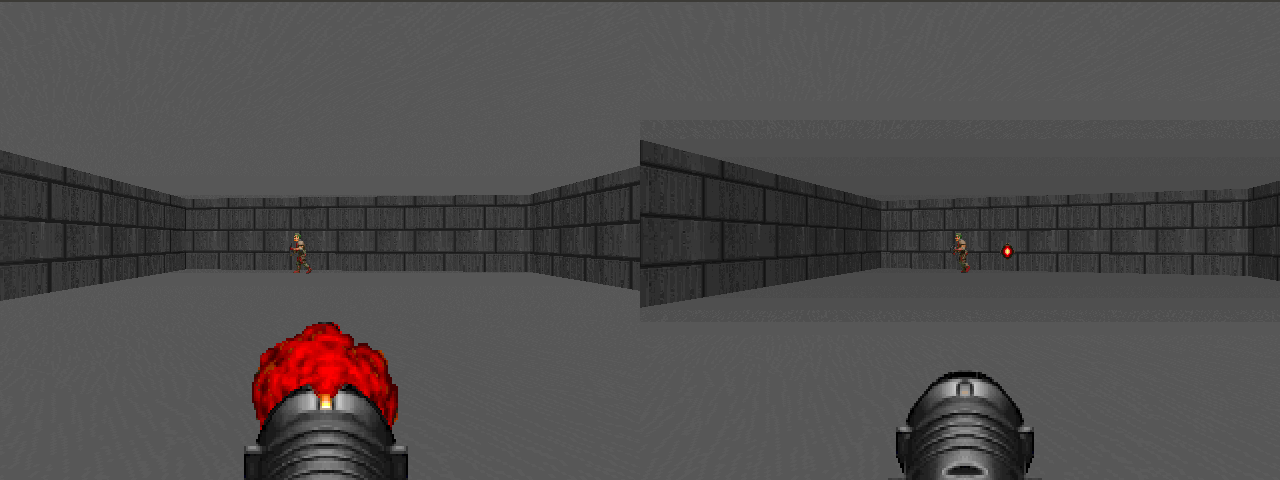
\includegraphics[scale=0.32]{predict_position.png}
			\caption{2 Doom gameplay frames from `predict position' scenario.}\label{fig:predict_position}
		\end{figure}
		\paragraph{Motivation} 
			The purpose of the scenario is teach agent to synchronize missle weapon shot (involving a signifficant delay between shooting and hitting) with target movements. Agent should be able to shoot so that missle and monster meet each other.

		\paragraph{Decription}
			The map is a rectangle room. Player is spawned along the longer wall, in the center. A monster is spawned randomly somewhere along the opposite wall and walks between left and right corners along the wall. Player is equipped with a rocket launcher and a single rocket. Episode ends when missle hits a wall/the monster or on timeout.
		\paragraph{Rewards}
		\begin{itemize}
			\item +1 for killing the monster
		\end{itemize}
		
		\paragraph{Suggested configuration}
		\begin{itemize}
			\item living reward =-0.0001
			\item available buttons: turn left, turn right, shoot (attack)
			\item timeout = 300
		\end{itemize}
	\newpage

	\subsection{Take Cover}
		\begin{figure}
			\centering
			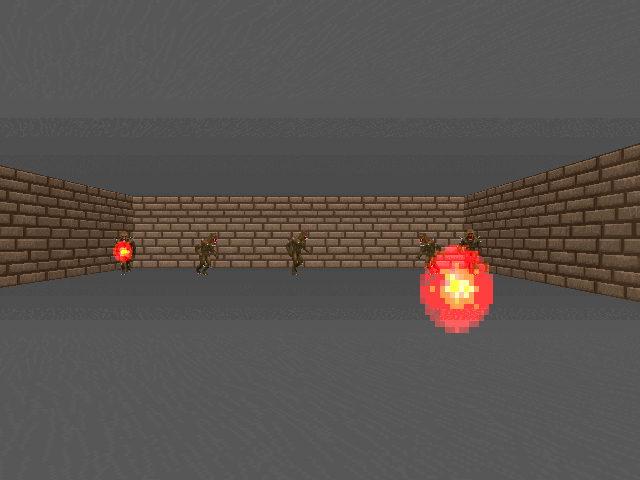
\includegraphics[scale=0.5]{take_cover.png}
			\caption{Doom gameplay frame from `take cover' scenario.}
		\end{figure}
		\paragraph{Motivation} 
			The purpose of this scenario is to teach agent to link incomming missles with his estimated lifespan. Agent should learn that being hit means a decrease in health and this in turn leads to death that is undesirable. In effect agent should learn how to avoid missles.

		\paragraph{Decription}
			Map is a rectangle. Player is spawned along the longer wall, in the center. A couple of fireball-spitting monsters are spawned randomly somewhere along the opposite wall and try to kill the player with fireballs. The player has no weapon and can only move sideways (config). More monsters appear with time. Episode ends when player dies which is inevitable.

		\paragraph{Suggested configuration}
		\begin{itemize}
			\item living reward = 1
			\item death penalty = 100
			\item 2 available buttons: move left, move right
		\end{itemize}
	\newpage


\section{Creating scenarios}\label{sec:creating_scenarios}
	\subsection{Rewards}
	In order to support reward it is neccessary to utilize global variable 0 in ACS script and it can be achieved by the following code:\\
	//TODO make it look like code \\
	global int 0:reward;\\
	Name given to the variable does not matter. Vizia will treat the variable as fixed point number ....bla bla bla going to bed. . .

	\subsection{User Variables}
		How to easily achieve some most common tasks in acs scripts which are not so obvious and~were used here.
		e.g. shaping rewards, infinite ammo, respawning, friendly monsters, 

\section{Resources}
\chapter{Experiment}

\section{Goal of the Experiment}
The main purpose of the experiment is to show that Reinforcement Learning from visual input is possible using Vizia Environment. 	
Additionally, the eperiments tries to check influence of frame skipping on learning process.

\subsection{Experiment's Design}
Experiment consists of testing agents on `basic' scenario that use different \emph{skiprate}. We define \emph{skiprate} as number of game frames that are skiped (ignored) by agent. Skipping a frame is acomplished with makeAction method  (see TODO /REF/) so rewards are acummulated and chosen action is extended for the skipped frames. Skiprate values of 0,1,2,3,4,5,6 and 7 are included in the experiment. 

For each skiprate, agent is to play for epochs. Each epoch requires performing 5000 learning steps, each involving making an action and running a learning update. After the learning portion of each epoch, 100 random test episodes are conducted and mean score is used for assessment.  

\section{Tested Agent's Design}
	The agent is heavily inspired by Google DeepMind Atari DQN \cite{mnih-dqn-2015}\cite{mnih-atari-2013} and is conceptually identical to DeepMind's algorithm. Game is modelled as Markov Decision Process and Q-learning\cite{watkins:mlj92} is used to reach the optimal policy. $\epsilon$-greedy policy with linear $\epsilon$ decay is used to choose actions. Additionally, a technique called experience replay\cite{mnih-dqn-2015} was applied. A convolutional Neural Network is used for approximation of q-values and it is trained with Backpropagation Algorithm\cite{lecun-98b} using Stochastic Gradient Descent with mini-batches. Agent is written in Python and uses Theano\cite{Bastien-Theano-2012}\cite{bergstra+al:2010-scipy} and Lasagne\cite{sander_dieleman_2015_27878} to implement neural networks.

\section{Experimental Setup} 
	\subsection{Operating System and Hardware}
	\begin{description}
		\item[Operating System] Linux Mint 17 x86\_64, kernel 3.13.0-24-generic
		\item[CPU] Intel Core i7-4790, 4x4GHz
		\item[GPU] GeForce GTX 970, 1664 CUDA cores, 4GB RAM
	\end{description}

	\subsection{Game Settings}
		The experiment uses the simplest scenario from the pool, that is the `basic' scenario (see \ref{subsec:basic}). Screen buffer consists of 3 channels (RGB) and resolution is 60x45 pixels.

	\subsection{Neural Network Architecture}
		Network architecture used for the experiment is rather small though it is suspected that it is still excesively robust for such a simple problem. The network consists of two convolutional layers with 32 square filters (7 and 4 pixels wide) each connected to a max-pooling layer with poolsize equal to 2 and rectifiers. Convolutional layers are followed by a fully connected layer with 800 leaky rectified linear units and output layer with 8 linear units coresponding to 8 available actions (combinations of 3 available buttons). 
	
	\subsection{Agent Parameters}
		\begin{itemize}
		\item $\gamma$ (discount factor) = 0.99
		\item learning rate = 0.01
		\item mini-batch size = 40
		\item initial $\epsilon$ = 1.0
		\item final $\epsilon$ = 0.1
		\item steps after which $\epsilon$ decay will start = 100000
		\item steps to fully decrease $\epsilon$ = 100000
		\item replay memory  capacity = 10000
		\end{itemize}
	

\section{Results}
	\subsection{Numerical Issues}
		In case of 0 skiprate a major numerical problem was euncountered. Estimated q-values very rapidly grew to to infinite vallues (in the first epoch) which prevented further learning. Quite unexpectedly, increasing resolution from 60x45 to 120x90 eliminated the problem at the cost of longer learning time. A faulty code is an obvious explenation, however none has been found yet therefore a conceptually oriented mechanism should be also considered. It is suggested that combination of 0 skiprate and low resolution may produce state transitions that incorporate barely distinguishible states. As a consequence each update would signifficantly infaltes q-values for each state and rapidly reach infinities.

		Because high number of epochs required to get fairly satisfying results with skiprate 0, learning was continued to see if it would follow the trend as expected. //TODO

	\subsection{Learning Quality}
		As seen in the Figure \ref{fig:results} all agents reached estimated maximum average score of ~80 or showed trend towards achieving this value. Watching agents play the scenario proved that agents in fact behave very reasonably. They move towards the target and shoot when it appears in front of them. Occasionally agents fire marginally too soon or stay idle (first available action) throughout whole episode. 

	\subsection{Skiprate} 
		As seen in the Figure \ref{fig:results} higher skiprate lead to quicker and smoother learning, which was expected as higher skiprate makes consequences of actions more immediate and easier to notice. It was also anticipated that higher skiprate would slightly lower scores due to lack of so small-grained control. As seen in Table \ref{tab:results} just the oposite is true and it is doubtful that too short training was the culprit since most of agents reach signifficant stability in 80 epochs and do not appear to be able to ever transcend current highscores.  //TODO (more prone to crazy behaviors)
	\begin{table}
		\begin{center}
			\begin{tabular}{ |l || c | r |}
				\hline
				Skiprate & Best epoch score & Mean of 10 best epochs \\ \hline
				0 & 74.17 & 72.679 \\ \hline
				1 & 77.84 & 76.187 \\ \hline
				2 & 79.35 & 77.914 \\ \hline
				3 & 80.98 & 78.695 \\ \hline
				4 & 81.8 & 80.755 \\ \hline
				5 & 81.32 & 80.162 \\ \hline
				7 & 81.08 & 80.496 \\ \hline
			\end{tabular}
		\end{center}
		\caption{Influence of skiprate on achieved highscores.}\label{tab:results}
	\end{table}

	\begin{figure}
		\centering
		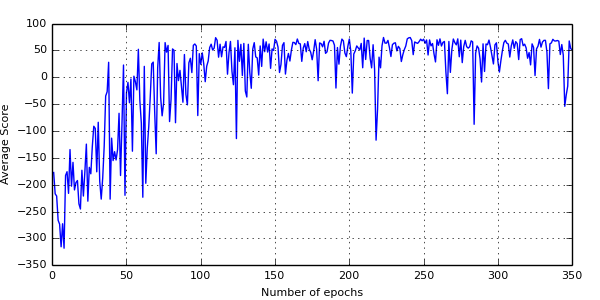
\includegraphics{results_skiprate0.png}
		\caption{Graphs showing mean performance of agent with zero skiprate throughout 350 learning epochs.}\label{fig:results_skiprate0}
	\end{figure}

	\begin{figure}
		\centering
		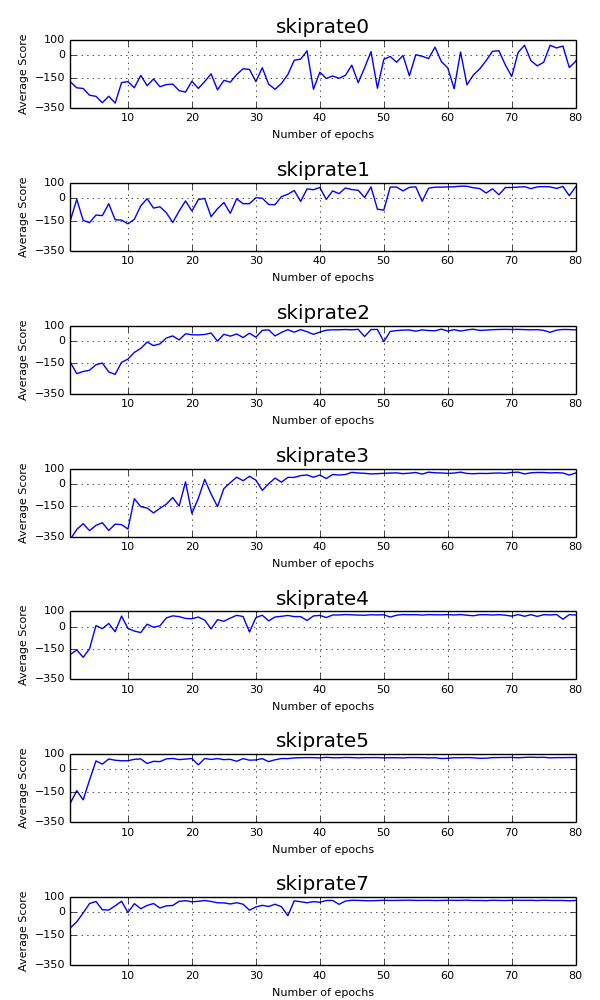
\includegraphics{results.png}
		\caption{Graphs showing mean performance of tested agent with different skip values throughout 80 learning epochs.}\label{fig:results}
	\end{figure}

\chapter{Framework}

\section{Achieved Goals}
\section{Future Work}



% Bibliography (books, articles) starts here.
\bibliographystyle{plain}{\raggedright\sloppy\small\bibliography{bibliography}}

% All appendices and extra material, if you have any.
\cleardoublepage\appendix%

\chapter{GitHub}
The thesis and VIZIA framework are available on the github server: \\
\url{https://github.com/Marqt/Vizia/}


\chapter{Building}
\section{Prerequisites}
\begin{itemize}
\item preferably Linux
\item cmake
\item make
\item gcc 4.??
\item Boost 
\item Python 2.6+ with Numpy and Boost.Python (for pyhon binding)
\item Java compiler (for Java binding)
\end{itemize}
\section{Before Building}
	In addition to prerequisites mentioned above, the following packages need to be install to build Zdoom itself:
	\begin{description}
		\item[Debian/Ubuntu:] \hfill \\
		sudo apt-get install build-essential zlib1g-dev libsdl2-dev libjpeg-dev nasm tar libbz2-dev libgtk2.0-dev cmake git libfluidsynth-dev libgme-dev libopenal-dev timidity
		\item[Fedora:] \hfill \\
		yum install gcc-c++ make zlib-devel SDL2-devel libjpeg-turbo-devel nasm tar bzip2-devel gtk2-devel cmake git fluidsynth-devel game-music-emu-devel	openal-soft-devel timidity++
		\item[Arch linux:] \hfill \\
		pacman -S --needed gcc make zlib sdl2 libjpeg-turbo nasm tar bzip2 gtk2 cmake git fluidsynth libgme fmodex openal timidity++
		\item[openSUSE:] \hfill \\
		zypper install gcc-c++ make zlib-devel libSDL2-devel libjpeg-devel nasm tar libbz2-devel gtk2-devel cmake git fluidsynth-devel libgme-devel openal-soft-devel timidity
	\end{description}
\section{Compilation}
To compile Vizia run this commands 
	\begin{lstlisting}
cmake -DCMAKE_BUILD_TYPE=Release
make all
	\end{lstlisting}
\chapter{Methods and Structures Handout}
\section{Methods}


\begin{clinee}
DoomGame::~DoomGame();
\end{clinee}


\begin{clinee}
bool DoomGame::init();
\end{clinee}


\begin{clinee}
bool DoomGame::loadConfig(std::string configFilePath);
\end{clinee}


\begin{clinee}
void DoomGame::addAvailableButton(Button button);
\end{clinee}

\begin{clinee}
void DoomGame::setButtonMaxValue(Button button, int maxValue);
\end{clinee}


\begin{clinee}
void DoomGame::addAvailableButton(Button button, int maxValue);
\end{clinee}


\begin{clinee}
void DoomGame::clearAvailableButtons();
\end{clinee}


\begin{clinee}
void DoomGame::addAvailableGameVariable(GameVariable var);
\end{clinee}


\begin{clinee}
void DoomGame::clearAvailableGameVariables();
\end{clinee}
	

\begin{clinee}
void DoomGame::addCustomGameArg(std::string arg);
\end{clinee}


\begin{clinee}
void DoomGame::clearCustomGameArgs();
\end{clinee}


\begin{clinee}
void DoomGame::setMode(Mode mode);
\end{clinee}
	

\begin{clinee}
void DoomGame::setDoomEnginePath(std::string path);
\end{clinee}


\begin{clinee}
void DoomGame::setDoomGamePath(std::string path);
\end{clinee}


\begin{clinee}
void DoomGame::setDoomScenarioPath(std::string path);
\end{clinee}


\begin{clinee}
void DoomGame::setDoomConfigPath(std::string path);
\end{clinee}


\begin{clinee}
void DoomGame::setDoomMap(std::string map);
\end{clinee}
	

\begin{clinee}      
void DoomGame::setDoomSkill(int skill);
\end{clinee}
	

\begin{clinee}    
void DoomGame::setEpisodeStartTime(unsigned int tics);
\end{clinee}


\begin{clinee}
void DoomGame::setEpisodeTimeout(unsigned int tics);
\end{clinee}


\begin{clinee}
void DoomGame::setLivingReward(double livingReward);
\end{clinee}


\begin{clinee}
void DoomGame::setDeathPenalty(double deathPenalty);
\end{clinee}
	

\begin{clinee}
void DoomGame::setScreenResolution(ScreenResolution resolution);
\end{clinee}


\begin{clinee}
void DoomGame::setScreenFormat(ScreenFormat format);
\end{clinee}
	

\begin{clinee}       
void DoomGame::setRenderHud(bool hud);
\end{clinee}


\begin{clinee}  
void DoomGame::setRenderWeapon(bool weapon);
\end{clinee}


\begin{clinee}  
void DoomGame::setRenderCrosshair(bool crosshair);
\end{clinee}


\begin{clinee}  
void DoomGame::setRenderDecals(bool decals);
\end{clinee}


\begin{clinee}  
void DoomGame::setRenderParticles(bool particles);
\end{clinee}


\begin{clinee}
void DoomGame::setWindowVisible(bool visibility);
\end{clinee}


\begin{clinee}
void DoomGame::setConsoleEnabled(bool console);
\end{clinee}
	

\subsection{Runtime Methods}\label{subsec:runtime_methods}
	

\begin{clinee}
void DoomGame::newEpisode();
\end{clinee}


\begin{clinee}
	void DoomGame::setAction(std::vector<int> const &actions);
\end{clinee}


\begin{clinee}
	void DoomGame::advanceAction(unsigned int tics, bool stateUpdate, bool renderOnly);
\end{clinee}


\begin{clinee}
	void DoomGame::advanceAction(unsigned int tics);
\end{clinee}


\begin{clinee}
	void DoomGame::advanceAction();
\end{clinee}


\begin{clinee}
	void DoomGame::advanceAction(unsigned int tics, bool stateUpdate, bool renderOnly);
\end{clinee}


\begin{clinee}
	double DoomGame::getLastReward();
\end{clinee}


\begin{clinee}
	double DoomGame::makeAction(std::vector<int> const &actions, unsigned int tics);
\end{clinee}

   
\begin{clinee}
	double DoomGame::makeAction(std::vector<int> const &actions);
\end{clinee}


\begin{clinee}
	DoomGame::State DoomGame::getState();
\end{clinee}


\begin{clinee}
	std::vector<int> DoomGame::getLastAction();
\end{clinee}


\begin{clinee}
	uint8_t * const getGameScreen();
\end{clinee}


\begin{clinee}
	int DoomGame::getGameVariable(GameVariable var);
\end{clinee}


\begin{clinee}
	double DoomGame::getSummaryReward();
\end{clinee}


\begin{clinee}
	bool DoomGame::isNewEpisode();
\end{clinee}


\begin{clinee}
	bool DoomGame::isEpisodeFinished();
\end{clinee}


\begin{clinee}
	void DoomGame::setSeed(unsigned int seed);
\end{clinee}


\begin{clinee}
	void DoomGame::close();
\end{clinee}


\begin{clinee}
	bool DoomGame::isRunning();
\end{clinee}


\begin{clinee}
	void DoomGame::sendGameCommand(std::string cmd);
\end{clinee}


\subsection{Query Methods}


\begin{clinee}
int DoomGame::getAvailableButtonsSize();
\end{clinee}

\begin{clinee}
int DoomGame::getAvailableGameVariablesSize();
\end{clinee}

\begin{clinee}
Mode DoomGame::getMode();
\end{clinee}

\begin{clinee}
double DoomGame::getLivingReward();
\end{clinee}

\begin{clinee}
double DoomGame::getDeathPenalty();
\end{clinee}

\begin{clinee}
unsigned int DoomGame::getEpisodeStartTime();
\end{clinee}

\begin{clinee}
unsigned int DoomGame::getEpisodeTimeout();
\end{clinee}

\begin{clinee}
unsigned int DoomGame::getEpisodeTime();
\end{clinee}

\begin{clinee}
int DoomGame::getScreenWidth();
\end{clinee}

\begin{clinee}
int DoomGame::getScreenHeight();
\end{clinee}

\begin{clinee}
int DoomGame::getScreenChannels();
\end{clinee}

\begin{clinee}
size_t DoomGame::getScreenPitch();
\end{clinee}

\begin{clinee}
size_t DoomGame::getScreenSize();
\end{clinee}

\begin{clinee}
ScreenFormat DoomGame::getScreenFormat();
\end{clinee}

\begin{clinee}
unsigned int DoomGame::getSeed();
\end{clinee}

\begin{clinee}
int DoomGame::getButtonMaxValue(Button button);
\end{clinee}

\section {Utility Functions}


\begin{clinee}
unsigned int DoomTics2Ms(unsigned int tics);
\end{clinee}


\begin{clinee}
unsigned int Ms2DoomTics(unsigned int ms);
\end{clinee}


\begin{clinee}
double DoomFixedToDouble(int doomFixed);
\end{clinee}


\section{Structures and Enumerations}\label{sec:appendix_structs_and_enums}
\subsection{State}

	
\begin{clinee}
	struct State {
	    unsigned int number; 
	    std::vector<int> gameVariables;
	    uint8_t * imageBuffer;
	};
\end{clinee}

\subsection{Mode}\label{subsec:mode}

\paragraph{Modes:}

\begin{itemize}
	\item PLAYER
	\item SPECTATOR
	\item ASYNC\_PLAYER 
	\item ASYNC\_SPECTATOR 
\end{itemize}

\subsection{ScreenFormat}\label{subsec:screenformat}


\textbf{ScreenFormats:}
\begin{itemize}
     \item CRCGCB 
     \item CRCGCBDB
     \item RGB24
     \item RGBA32
     \item ARGB32
     \item CBCGCR
     \item CBCGCRDB
     \item BGR24
     \item BGRA32
     \item ABGR32
     \item GRAY8
     \item DEPTH\_BUFFER8
     \item DOOM\_256\_COLORS8
\end{itemize}
\subsection{ScreenResolution} \label{subsec:screenresolution}


\textbf{ScreenResolutions:}
\begin{itemize}
    \item RES\_40X30
    \item RES\_60X45
    \item RES\_80X50
    \item RES\_80X60
    \item RES\_100X75
    \item RES\_120X75
    \item RES\_120X90
    \item RES\_160X100
    \item RES\_160X120
    \item RES\_200X120
    \item RES\_200X150
    \item RES\_240X135
    \item RES\_240X150
    \item RES\_240X180
    \item RES\_256X144
    \item RES\_256X160
    \item RES\_256X192
    \item RES\_320X200
    \item RES\_320X240
    \item RES\_400X225
    \item RES\_400X300
    \item RES\_480X270
    \item RES\_480X360
    \item RES\_512X288
    \item RES\_512X384
    \item RES\_640X360
    \item RES\_640X400
    \item RES\_640X480
    \item RES\_720X480
    \item RES\_720X540
    \item RES\_800X450
    \item RES\_800X480
    \item RES\_800X500
    \item RES\_800X600
    \item RES\_848X480
    \item RES\_960X600
    \item RES\_960X720
    \item RES\_1024X576
    \item RES\_1024X600
    \item RES\_1024X640
    \item RES\_1024X768
    \item RES\_1088X612
    \item RES\_1152X648
    \item RES\_1152X720
    \item RES\_1152X864
    \item RES\_1280X720
    \item RES\_1280X854
    \item RES\_1280X800
    \item RES\_1280X960
    \item RES\_1280X1024
    \item RES\_1360X768
    \item RES\_1366X768
    \item RES\_1400X787
    \item RES\_1400X875
    \item RES\_1400X1050
    \item RES\_1440X900
    \item RES\_1440X960
    \item RES\_1440X1080
    \item RES\_1600X900
    \item RES\_1600X1000
    \item RES\_1600X1200
    \item RES\_1680X1050
    \item RES\_1920X1080
    \item RES\_1920X1200
    \item RES\_2048X1536
    \item RES\_2560X1440
    \item RES\_2560X1600
    \item RES\_2560X2048
    \item RES\_2880X1800
    \item RES\_3200X1800
    \item RES\_3840X2160
    \item RES\_3840X2400
    \item RES\_4096X2160
    \item RES\_5120X2880
\end{itemize}

\subsection{GameVariable} \label{subsec:gamevar}


\textbf{Game Variables:}
\begin{itemize}
    \item KILLCOUNT
    \item ITEMCOUNT
    \item SECRETCOUNT
    \item FRAGCOUNT
    \item HEALTH
    \item ARMOR
    \item DEAD
    \item ON\_GROUND
    \item ATTACK\_READY
    \item ALTATTACK\_READY
    \item SELECTED\_WEAPON
    \item SELECTED\_WEAPON\_AMMO
    \item AMMO0
    \item AMMO1
    \item AMMO2
    \item AMMO3
    \item AMMO4
    \item AMMO5
    \item AMMO6
    \item AMMO7
    \item AMMO8
    \item AMMO9
    \item WEAPON0
    \item WEAPON1
    \item WEAPON2
    \item WEAPON3
    \item WEAPON4
    \item WEAPON5
    \item WEAPON6
    \item WEAPON7
    \item WEAPON8
    \item WEAPON9
    \item USER1
    \item USER2
    \item USER3
    \item USER4
    \item USER5
    \item USER6
    \item USER7
    \item USER8
    \item USER9
    \item USER10
    \item USER11
    \item USER12
    \item USER13
    \item USER14
    \item USER15
    \item USER16
    \item USER17
    \item USER18
    \item USER19
    \item USER20
    \item USER21
    \item USER22
    \item USER23
    \item USER24
    \item USER25
    \item USER26
    \item USER27
    \item USER28
    \item USER29
    \item USER30
\end{itemize}

\subsection{Button} \label{subsec:button}


\textbf{Buttons:}
\begin{itemize}
    \item ATTACK
    \item USE
    \item JUMP
    \item CROUCH
    \item TURN180
    \item ALTATTACK
    \item RELOAD
    \item ZOOM
    \item SPEED
    \item STRAFE
    \item MOVE\_RIGHT
    \item MOVE\_LEFT
    \item MOVE\_BACKWARD
    \item MOVE\_FORWARD
    \item TURN\_RIGHT
    \item TURN\_LEFT
    \item LOOK\_UP
    \item LOOK\_DOWN
    \item MOVE\_UP
    \item MOVE\_DOWN
    \item LAND
    \item SELECT\_WEAPON1
    \item SELECT\_WEAPON2
    \item SELECT\_WEAPON3
    \item SELECT\_WEAPON4
    \item SELECT\_WEAPON5
    \item SELECT\_WEAPON6
    \item SELECT\_WEAPON7
    \item SELECT\_WEAPON8
    \item SELECT\_WEAPON9
    \item SELECT\_WEAPON0
    \item SELECT\_NEXT\_WEAPON
    \item SELECT\_PREV\_WEAPON
    \item DROP\_SELECTED\_WEAPON
    \item ACTIVATE\_SELECTED\_ITEM
    \item SELECT\_NEXT\_ITEM
    \item SELECT\_PREV\_ITEM
    \item DROP\_SELECTED\_ITEM
    \item LOOK\_UP\_DOWN\_DELTA
    \item TURN\_LEFT\_RIGHT\_DELTA
    \item MOVE\_FORWARD\_BACKWARD\_DELTA
    \item MOVE\_LEFT\_RIGHT\_DELTA
    \item MOVE\_UP\_DOWN\_DELTA
\end{itemize}

\section{Exceptions}\label{sec:appendix_exception}
\begin{itemize}
    \item SharedMemoryException
    \item MessageQueueException
    \item DoomErrorException
    \item DoomUnexpectedExitException
    \item DoomIsNotRunningException
    \item PathDoesNotExistsException
\end{itemize}




% Colophon is a place where you should let others know about copyrights etc.
\ppcolophon

\end{document}
